\chapter{Families of Hidden Markov Models}
\index{Families of Hidden Markov Models@\emph{Families of Hidden Markov Models}}\label{hmmfamily}

One basic technique for aligning a sequence to an existing backbone alignment is to build an HMM on the backbone alignment, and then align the sequence to the HMM.  In Section~\ref{hmmfamily:algorithm}, I present a new technique called \emph{families of HMMs} that allows accurate alignment of divergent sequences.  In Section~\ref{hmmfamily:modification}, I describe the technical details of the algorithms and the modifications necessary for the algorithm to be applied to phylogenetic placement, metagenomic analyses, and ultra-large alignment estimation.

\section{Families of HMM}\label{hmmfamily:algorithm}
The families of HMMs (fHMMs) is a technique for aligning a query sequence to a backbone alignment.  This technique was originally developed to address the problem of phylogenetic placement, specifically, how to best align a short fragmentary read to an existing backbone alignment, and then use that alignment to insert the query sequence into a backbone tree.  However, we quickly realized that the fMMs can be applied to problem in which a query sequence of any length is needed to be aligned to an existing alignment.

The basic outline of the fHMMs is to divide the backbone alignment into subalignments of closely related sequences.  The fHMMs are comprised of the HMMs computed on each of the subalignments.  To align a query sequence, the query sequence is aligned against each HMM; each alignment yields a \emph{bit score}, which is a measure of the quality of the match between the query sequence and the HMM. We select the HMM that yields the best bit score match to the query sequence, and we align the query sequence to the HMM.  This alignment, by transitivity, defines the alignment of the query sequence to the entire backbone alignment.  The creation of the HMM, scoring of the query sequence against the HMMs, and alignment of the query sequence against the HMM use the software suite in HMMER3~\cite{hmmer}.  The commands used for each step are shown in Section~\ref{hmmfamily:modification}.
%\textbf{Nam:Set up one section in the appendix that contains *ALL* commands used for each study.}

I now provide the details of each step.

\paragraph{Building the families of HMM.}
We apply the recursive decomposition technique called the 
``centroid edge decomposition'' \cite{Liu2012} 
to build the family of HMMs (see Fig.~\ref{hmmfamily:decomp}).  
From the backbone tree, we select the centroid edge $e$ 
(one whose removal separates the leaf set into 
approximately two equally 
sized subsets).
We remove $e$ (but not its endpoints) from 
the backbone tree  to produce two subtrees.  
This process is recursively repeated on each subtree with
more leaves than a user-defined threshold $t$.  Thus, at the end
of the decomposition, each subtree has $t$ or fewer leaves, and the leaf set of each subtree defines subset.
The backbone alignment restricted to each of these subsets is
called a ``subset alignment".  For each alignment subset, we run HMMBUILD to produce an HMM, producing a match state for every site that is not completely gapped. 
 
\begin{figure}[htbp]
\centering
{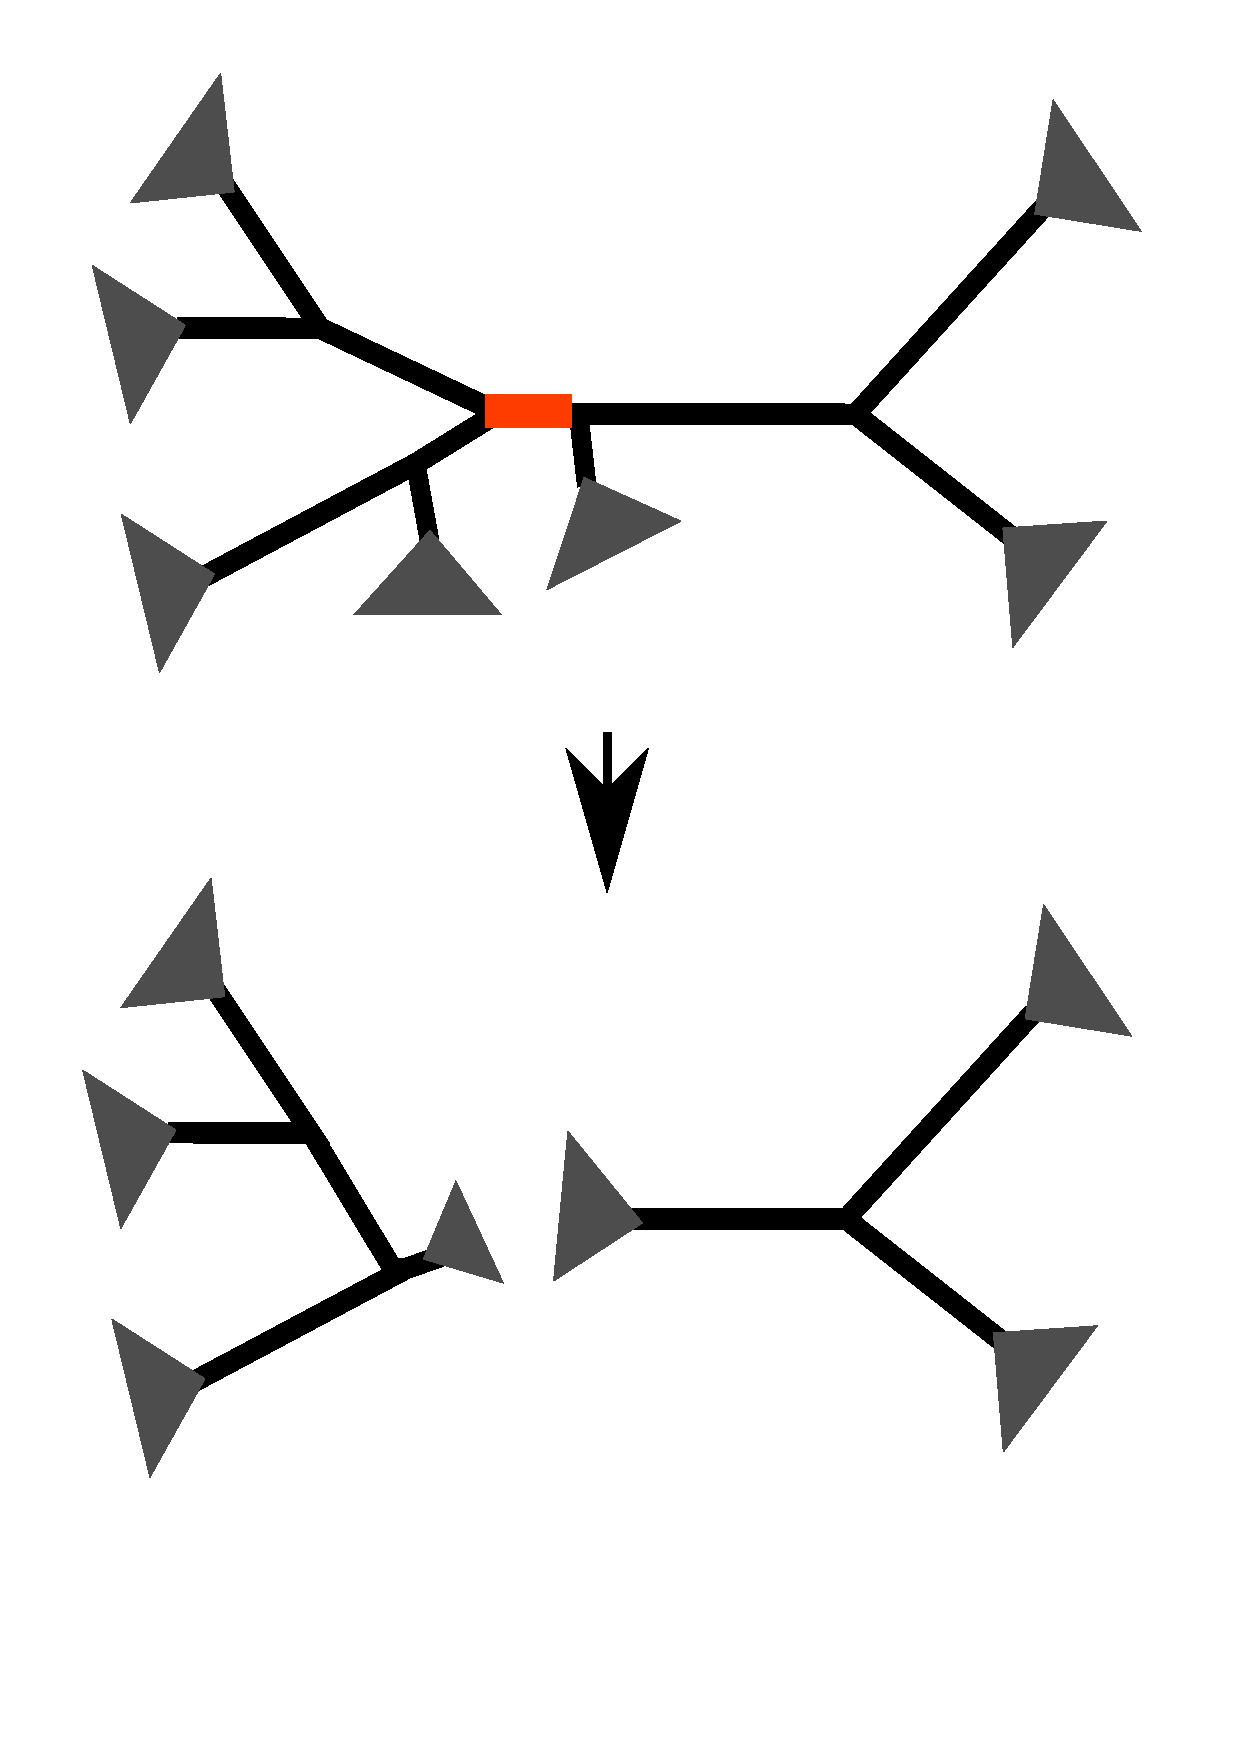
\includegraphics[width=.50\textwidth]{hmmfamily/decomposition}}
\caption[Example of centroid decomposition.]{Example of centroid decomposition.  The centroid edge (colored orange) partitions the tree into roughly two equally sized subtrees.  This edge is removed, and two subtrees are created.  This process is recursively repeated on the subtrees until all subtrees contain at most as many sequences as a user-set threshold.} 
\label{hmmfamily:decomp}
\end{figure}


\paragraph{Aligning the query sequences.}
For a given query sequence $q$, it is scored against each of the HMMs using HMMSEARCH, which reports a HMMER ``bit score'', a measure of the quality of the match between the query sequence $q$ and the HMM (see Fig.~\ref{hmmfamily:alignment}).  The HMM that yields the best bit score is selected and an extended subalignment is produced by inserting $q$ into the subalignment using HMMALIGN.  The alignment of $q$ to the entire backbone alignment is computed through transitivity (see Fig.~\ref{hmmfamily:trans}).

In the special case where a query sequence resulted in no scores against any of the HMMs (i.e., HMMSEARCH reports the sequence as non-homologous to all HMMs), the query sequence is omitted from the final alignment.  

\begin{figure}[htbp]
\centering
{
\includegraphics[width=1.0\textwidth]{hmmfamily/alignment}}
\caption[Example of alignment using HMM families.]{Example of aligning a query sequence using the families of HMMs.  The traditional approach uses a single HMM to align the query sequence.  In the fHMMs appraoch, the query sequence is scored against all HMMs.  The HMM that yields the best bit score, HMM-3 in this case, is selected and the query sequence is aligned to the HMM.} 
\label{hmmfamily:alignment}
\end{figure}

\begin{figure}[htbp]
\centering
{
\includegraphics[width=1.0\textwidth]{hmmfamily/alignment}}
\caption[Example of alignment of query sequence through transitivity.]{Example of extending the alignment of query sequence to the full backbone alignment through transitivity.  \textbf{Fix this figure, it should show transitivity merger, but I overwrote the image with decomposition.  Original picture is still on home desktop}.} 
\label{hmmfamily:trans}
\end{figure}


\section{Technical details}\label{hmmfamily:modification}
\paragraph{Backbone alignment and tree.}  The quality of the fHMMs is heavily dependent on the quality of the backbone alignment and tree.  Thus, it is vital that an accurate method is used to estimate the backbone alignment and tree
\paragraph{Decomposition threshold.}
\paragraph{HMM commands.}



% \section{Motivation}\label{hmmfamily:motivation}
% There exists many databases containing structurally-based alignments that have been manually curated~\cite{Cannone2002,Thompson1999,Punta2012}.  One advantage of using a manually curated alignment is that manual curation can preserve conserved structures that may not be preserved by typically alignment methods.  However, because manual curation requires a large investment of time, the curated alignments often contain small number of sequences.  Thus, one technique for generating a larger alignment from a manually curated alignment is to use the curated alignment as a backbone alignment, and the remaining sequences are aligned to the backbone alignment.  
% 
% An example of this approach is within Pfam~\cite{Punta2012}.  Each protein family consists of a seed alignment, a manually-curated alignment.  A HMM is computed on the seed alignment, and the remaining sequences in the protein family are aligned to the HMM to obtain an alignment on the entire protein family.  Often times, the protein family can span from a very diverse range of species.  Thus, the HMM may have difficulty representing an alignment from very evolutionarily divergent species.
% 
% In order to explore this issue, I examined an application of the HMM alignment approach under the context of \emph{phylogenetic placement}.  The ``phylogenetic placement" problem is formally stated as follows:
% 
% \noindent{\em Phylogenetic Placement Problem. }
% \begin{itemize}
% \item Input: the {\em backbone} tree $T$ and alignment $A$ on set $S$ of full-length sequences,
% and query sequence $s$.
% \item Output: tree $T'$ containing $s$ obtained by adding $s$ as a leaf to
% $T$.
% \end{itemize}
% 
% The evolutionary relationship between the query sequence and the full-length sequences can be inferred from the placement location of the query sequence in the tree.
% 
% Methods for the first step 
% include HMMALIGN\cite{Eddy1998}
% and PaPaRa\cite{Berger2011a} method.  
% Methods for the second step include 
%  EPA\cite{Berger2011} and pplacer\cite{Matsen2010}, which
% seek to optimize maximum likelihood
% (pplacer also provides a Bayesian approach).
% Methods for phylogenetic placement can therefore
% be described
% by how they handle each step.
% Three such methods
% include PaPaRa+EPA\cite{Berger2011a},
% HMMALIGN+EPA\cite{Berger2011},
% and HMMALIGN+pplacer\cite{Matsen2010}.
% EPA and pplacer are comparably 
% fast and have almost identical 
% placement accuracy,
%   but have somewhat different memory usage and algorithmic features\cite{Matsen2010};
% hence the differences between HMMALIGN+EPA and HMMALIGN+pplacer
% do not impact the placement accuracy, and have a minor
% impact on running time and memory usage.
% The two techniques for computing the extended alignment,
% PaPaRa and HMMALIGN, are very different.
% HMMALIGN computes a HMM to represent the full-length alignment,
% and then aligns each query sequence to that HMM.  In contrast,
% PaPaRa uses RAxML to estimate ancestral state 
% vectors for each branch in the
% tree, aligns the query sequence to every ancestral state
% vector, selects the alignment that had the best score and uses
% it to extend
% alignment $A$ to include $s$.
% Consequently, PaPaRa is computationally more 
% expensive than HMMALIGN\cite{Berger2011a}, but EPA placements
% of query sequences based upon PaPaRa extended alignments can be
% more accurate than EPA placements based upon HMMALIGN extended alignments.
% However, the improvement in topological accuracy reported\cite{Berger2011a}  for
% PaPaRa+EPA over HMMALIGN+EPA was
% relatively small, with PaPaRa+EPA placing
% query sequences on average
% about one edge closer to the correct
% location, out of 799 edges. 
% Therefore, PaPaRa+EPA and HMMALIGN+EPA are very close
% in terms of placement accuracy, although substantially different
% in terms of running time.
% 
% 
% We investigated the performance of HMMALIGN+pplacer on datasets simulated under 3 different model conditions
% with varying rates of evolution from~\cite{Liu2011}.  Each dataset originally consisted of 1000 full-length sequences.  Each dataset was randomly split in half into a query set and a backbone set, each containing 500 sequences.  For each sequence in the query set, 10 different fragments were simulated from the query sequence by selecting a random substring from the query sequence.  On the backbone set, a backbone alignment and tree were estimated using SAT\'{e}-II~\cite{Liu2011}.  We measured the placement accuracy of each query sequence by computing the \emph{delta error}, which is the difference in the number of missing edges of the backbone tree and the backbone tree after the query sequence is inserted into the backbone tree.  
% 
% On each dataset, we ran HMMALIGN+pplacer as follows.  An HMM is computed using HMMBUILD on the backbone alignment.  For each query sequence, the extended alignment of the query sequence is estimated by aligning the query sequence to the HMM using HMMALIGN.  Finally, the query sequence is inserted into backbone tree using pplacer.
% 
% Figure~\ref{sepp:initial} shows that under
% low rates of evolution, both HMMALIGN+pplacer yield very accurate
% placements (less than 0.01 delta error), however, as the datasets undergo higher rates of evolution, the accuracy degrades rapidly.
% 
% \begin{figure}[htbp]
% \centering
% {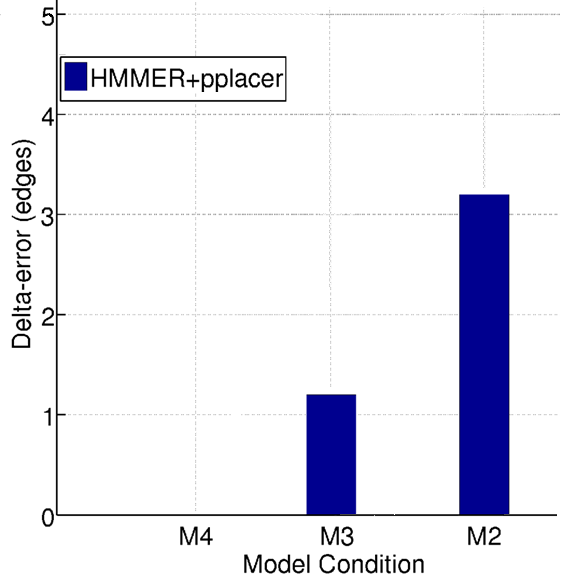
\includegraphics[width=0.60\textwidth]{hmmfamily/hmmer_pplacer}}
% \caption[HMMALIGN+pplacer on datasets of varying rates of evolution.]{Comparison of HMMALIGN+pplacer under 3 different model conditions, ranked in order of increasing rate of evolution.  Thus, M4 is the slowest evolving dataset, and M2 is the fastest evolving dataset.  The number of sequences in the backbone set is 500 for all model conditions.} 
% \label{sepp:initial}
% \end{figure}
% 
% In ~\cite{Liu2009}, Liu et al. developed a new alignment and phylogeny co-estimation technique that showed significantly improved alignment and tree reconstruction accuracy on simulated datasets under high rates of evolution (Fig.~\ref{hmmfamily:sate}).  For model conditions simulated under low rates of evolution, all alignment methods had comparable performances.  As the rates of evolution increased, however, alignment and tree accuracy degraded.  This observation lead to the key insight used within \sate: if the evolutionary distance of the sequences could be constrained, then better alignments could be estimated.  By dividing the sequences into subsets of closely related sequences, the evolutionary diameter of the individual subsets is reduced, and more accurate alignments can be estimated on each subset.  The subsets are created using the phylogeny such that sequences that are more closely related will typically fall into the same subset.  This divide-and-conquer approach serves as the basis of the \emph{family of HMM} technique.
% 
% \begin{figure}[htbp]
% \centering
% {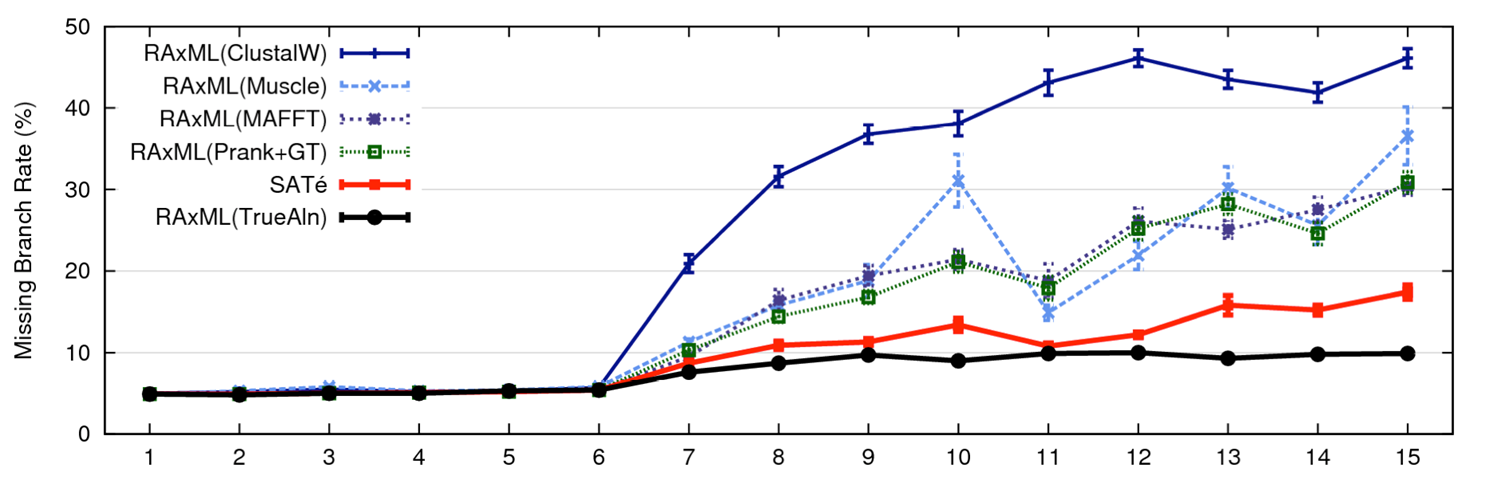
\includegraphics[width=1.00\textwidth]{sepp/sate}}
% \caption[Tree error of RAxML trees estimated on different alignment methods.]{Missing branch rate of RAxML trees estimated on different alignment methods under different model conditions (taken from \cite{Liu2009}).  Each model condition was ranked by difficulty; the higher the model condition number, the more evolution has taken place.} 
% \label{hmmfamily:sate}
% \end{figure}

